\chapter{Coupling Eulerian and Lagrangian Method}
\label{ch:coupling}

% chapter outline
% summarize previous chapters with references
%\section{Introduction to Hybrid Eulerian-Lagrangian \\Vortex Particle Method}

Chapter \ref{ch:helvpm} provided a detailed summary on Hybrid Eulerian-Lagrangian Vortex Particle Method, where we introduced the concept of coupling the Lagrangian and the Eulerian method. The chapter investigated the coupling algorithm without Schwartz iterative method used by Daeninck \cite{Daeninck2006}, and the Lagrangian correction algorithm used by Stock \cite{Stock2010a}. However, during the investigation and implementation of the algorithms, we observed some issues that had to be dealt with.

\section{Modifications to the Lagrangian Correction Strategy}
\label{seec:coupling-mthlcs}
The Lagrangian correction step by Stock \cite{Stock2010a}, based on the coupling strategy of Daeninck \cite{Daeninck2006} had to be modified in the present work. During the investigation of the algorithm, it became apparent that without additional steps, the total circulation in the Lagrangian method will be not be conserved.

The two issues that causes an error in the total circulation (and subsequently introduces additional error in the coupling) are the following:
	\begin{itemize}
	\item \textbf{Vortex particle re-initialization}: In section \ref{subsec:vortexBlobInitialization}, we observed that initializing the particles using the local particle volume and local vorticity causes a diffusive effect on the vorticity distribution due to the \textit{smoothing error} of Gaussian kernels. Section 	\ref{subsec:coupling-vpri} elaborates the cause and correction required for this problem.
	
	\item \textbf{Circulation of Vortex sheet}: In section \ref{sec:boundaryConditions}, we saw that as the vortex panel problem is singular, we require an additional constraint on total circulation of the vortex sheet. It is an unknown and has to be determined from the solution of the Eulerian method. Section \ref{subsec:coupling-covs} elaborates the methodology for determining the strength.
	\item \textbf{Conservation of total circulation}: The Lagrangian correction step, consisting of re-initializing the vortex blobs inside the interpolation domain $\Omega_I$ (Figure \ref{fig:interpolationDomainDefinition}), and the transfer of circulation to the vortex panels must ensure that the total circulation in the Lagrangian method is conserved. Section \ref{subsec:coupling-cotc} elaborates the methodology used to explicitly ensure the conservation of circulation in the Lagrangian domain during the correction step.
	\end{itemize}

	\subsection{Vortex Particle Re-initialization}
	\label{subsec:coupling-vpri}
	
	The Lagrangian correction step requires the correction (or adjustment/modification) of the strength of the vortex particles inside the interpolation domain $\Omega_{I}$, shown in Figure \ref{fig:interpolationDomainDefinition}.
	However, when investigating this approach, it becomes apparent that the standard initializing approach of local particle volume and local vorticity is erroneous.
		
	\subsubsection*{Concern with re-initialization method}

	%To understand the origin of the error, lets assume that the Eulerian vorticity solution $\omega$ used to initialize the Lagrangian particles is nearly exact. 

	The Lagrangian method discretizes the exact vorticity field $\omega$ by linear combination of $N$ Gaussian basis functions, i.e vortex blobs. Let $\mathcal{P} = \{1,...,N\}\subset\mathbb{N}$ be the set of particle indices of $N$ particles $p$ with position $\mathbf{x}_p$. The discrete continuous vorticity field $\hat{\omega}$ is given as,
		\begin{equation}
		\omega \approx \hat{\omega}(\mathbf{x}) = \sum_{p\in\mathcal{P}} \alpha_p \zeta_{\sigma}(\mathbf{x} - \mathbf{x}_p).
		\label{eq:coupling-mollifiedVorticityDistributionEquation}
		\end{equation}
	where $\alpha_p$ is the strength of particle $p\in\mathcal{P}$. In vortex method, it is typically a standard approach to initialize the particle strengths $\alpha_p$ using the local particle area $h^2$ and the local vorticity $\omega$,
		\begin{equation}
		\alpha_p = \omega_p\cdot{h^2}.
		\label{eq:coupling-standardInitialization}
		\end{equation}
	
	where $\omega_p$ is the vorticity at particle position $\mathbf{x}_p$. This approach was also employed by Stock \cite{Stock2010a}, to modify the strengths of the vortex blobs inside the correction region $\Omega_I$. However, in section \ref{subsec:vortexBlobInitialization}, we observed that this type of initialization introduces a \textit{smoothing error}. Barba and Rossi \cite{Barba2010a} noticed that the standard initialization corresponds to a Gaussian blurring of the original vorticity field and is equivalent to the ``diffusion" of the vorticity. 
	
	The accurate re-initialization of the Lagrangian vorticity field $\hat{\omega}^L$ in $\Omega_I$ using the Eulerian vorticity field $\omega^E$ must satisfy the following equality:
		\begin{equation}
		\omega^E = \hat{\omega}^L \qquad \mathrm{in}\ \Omega_I.
		\label{eq:coupling-eqa1}
		\end{equation} 
	Satisfying equation \ref{eq:coupling-eqa1} ensures that the vorticity solution of the Eulerian method $\omega^E$ matches the blurred (mollified) Lagrangian vorticity field $\hat{\omega}^L$. Substituting equation \ref{eq:coupling-mollifiedVorticityDistributionEquation} into Equation \ref{eq:coupling-eqa1} gives:
		\begin{equation}
		\omega^E(\mathbf{x}_j) = \sum_{i=p\in\mathcal{P}} \alpha_i \zeta_{\sigma}(\mathbf{x}_j - \mathbf{x}_i) \qquad \mathrm{in}\ \Omega_I, 
		\end{equation}
	simplifying to a system of linear equations,
		\begin{equation}
		\omega^E = \mathbf{A}_{ij}\alpha_i \qquad \mathrm{in}\ \Omega_I
		\label{eq:coupling-initialization}
		\end{equation}
	where $\mathbf{A}_{ij}=\zeta_{\sigma}(\mathbf{x}_j-\mathbf{x}_i)$ is a coefficient matrix. Therefore the strengths of the particles $\alpha_p$ must be obtained from equation \ref{eq:coupling-initialization} and the initialization of the particles using equation \ref{eq:coupling-standardInitialization} is mathematically incorrect. 
	
	Equation \ref{eq:coupling-initialization} is a linear system of equations equating the strengths of each particle to the desired Eulerian vorticity distribution. However, inverting the matrix $\mathbf{A}$ is still an open equation in vortex method, as stated by Koumoutsakos and Cottet \cite{Cottet2000a}, and was investigated by Barba and Rossi \cite{Barba2010a}. The problem is that the matrix $\mathbf{A}$ is full and badly condition for direct inversion. For a global field interpolation (i.e for unbounded domain), one could use Beale's iterative method which uses a \printAcron{successive over-relaxation}{SOR} for solving the equation \ref{eq:coupling-initialization}. This method relies on iterative correction of all the particles in the full Lagrangian domain. However, in our case for initializing the strengths of the particles only in the sub-domain $\Omega_{I}$ of the Lagrangian domain $\Omega_L$, it would require us to modify the strength of only those particles. In such case, Beale's iterative method is not valid and cannot be used. Therefore, Beale's method cannot be used to solve the problem of smoothing error.

	In future, the key to solving this smoothing error might be in the research works of Barba and Rossi \cite{Barba2010a}, where they try to reverse the blurring of the vorticity field by reversing the ``diffusion" caused by the smoothing kernel. However, currently for our investigation the best solution is to minimize the error in equation \ref{eq:coupling-standardInitialization}.

	\subsubsection*{Modification}

	The error $\epsilon$ due to the mismatch in the Eulerian vorticity field $\omega^E$ and the Lagrangian vorticity $\hat{\omega}^L$ in the interpolation domain $\Omega_I$ is defined as,
			\begin{equation}
			\epsilon = |\omega^E - \hat{\omega}^L| \qquad \mathrm{in}\ \Omega_I
			\label{eq:coupling-errorDefinition}
			\end{equation}
	where the error is divided into,
			\begin{equation}
			\epsilon = \epsilon_{\sigma} + \epsilon_h,
			\label{eq:coupling-totalError}
			\end{equation}
	the sum of the smoothing error $\epsilon_{\sigma}$, and the discretization error $\epsilon_h$. In section \ref{subsubsec:convergenceInterpolation}, we investigated the minimization of this error and observed that the error $\epsilon$ scales with particle resolution. With an overlap ratio of $\lambda=1$ and a small particle core spreading $\sigma$, we can ensure that the initialization error inside the interpolation domain $\Omega_I$ is minimal. To determined an appropriate core spreading $\sigma$, we should target an initialization error of $\epsilon\leqslant5\%$ ensuring a small error in coupling.
	
	\subsection{Circulation of Vortex sheet}
	\label{subsec:coupling-covs}
	
	The second concern with the implementation of Daeninck's coupling strategy and Stock's Lagrangian correction step is the uncertainty of the vortex sheet strengths. In section \ref{subsec:hybrid-ca}, we described that to time march the Lagrangian solution from $t_n$ to $t_{n}+\Delta t_L$, we have to enforce a \textit{no-slip} boundary condition at the wall by computing the satisfactory vortex sheet distribution $\gamma$. 
	
	To solve for the vortex sheet distribution $\gamma$ that satisfy the no-slip boundary conditions, we discretized the boundary integral equation using vortex panels, as described in section \ref{sec:boundaryConditions}. Koumoutsakos \cite{Koumoutsakos1993b}, related the vortex sheet strengths to the no-slip boundary conditions with Fredholm integral equation of the second kind, equation \ref{eq:fredholmIntegral2ndKind}. However, as this equation is singular, we require an additional constraint to obtain a unique solution. Kelvin's circulation theorem imposes a direct constraint on the integral strengths of the vortex sheet, shown in equation \ref{eq:circulationConstraintonPanels}, and can be used to find the unique solution. 
	
		\begin{figure}[!t]
		\centering
		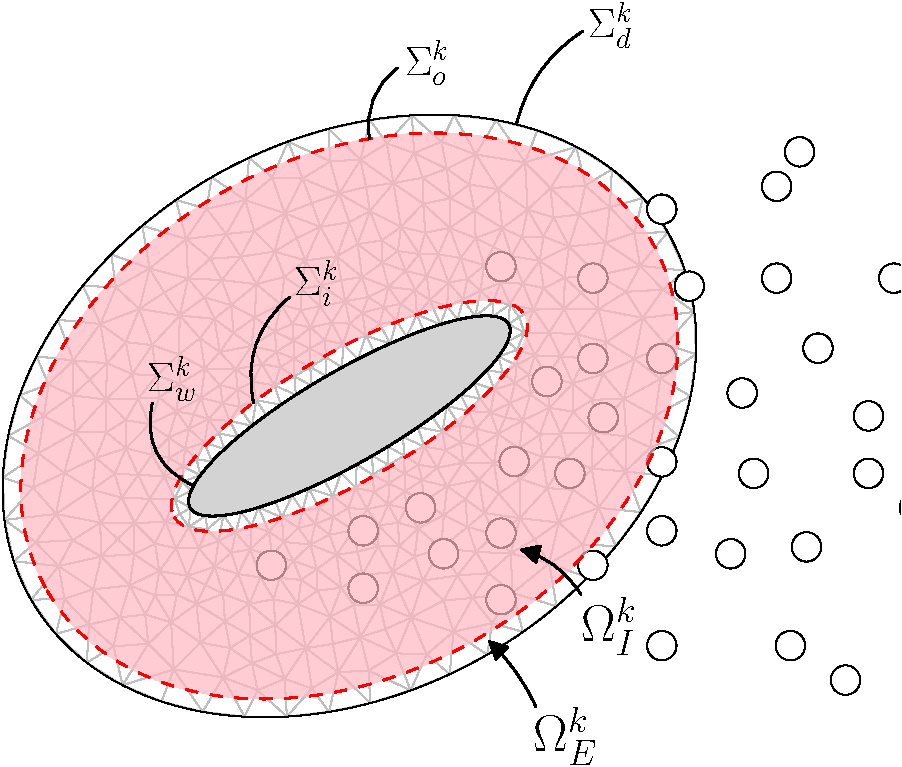
\includegraphics[width=0.5\linewidth]{./figures/coupling/modifiedDomain/domainDecomposition_kthDomain-crop.pdf}
		\caption{A domain decomposition with $k={1,...,N_E}$ Eulerian subdomains. The figure shows the definition of the $k^{\mathrm{th}}$ interpolation domain $\Omega_I^k$ belonging to the $k^{\mathrm{th}}$ Eulerian domain $\Omega_E^{k}$.}
		\label{fig:domainDecomposition_kthDomain}
		\end{figure}	

	Let us investigate a hybrid problem with $N_E$ number of Eulerian subdomain and the $k^{\mathrm{th}}$ Eulerian domain $\Omega_E^k\subset\Omega_L$ is defined as shown in Figure \ref{fig:domainDecomposition_kthDomain}. Stock \cite{Stock2010a} said that the Eulerian solution is assumed to be correct from the body surface $\Sigma_w^k$ to only somewhat inside of the outer Eulerian domain $\Sigma_d^k$. More precisely, all the Eulerian solution within the domain $\Omega_{in}^k$ with $\partial\Omega_{in}^k = \Sigma_o$ as shown in Figure \ref{fig:domainDecomposition_correctionDomains}. During the Lagrangian correction step, Stock corrected the particles $p$ with $\mathbf{x}_p\in\Omega_I^k$ using the more accurate Eulerian solution. So, any remaining Eulerian solution within $\Sigma_o^k$ that was not transfered during the Lagrangian correction step should be resolved by the vortex sheet to ensure conservation of circulation.
	
	In terms of circulation, we require that the Eulerian circulation $\Gamma_{in}^{E,k}$ and the corrected Lagrangian circulation $\hat{\Gamma}_{in}^{L,k}$ of the $k^{\mathrm{th}}$ correction region $\Omega_{in}^k$ must match to ensure conservation of circulation during the correction step, given by,
		\begin{equation}
		\Gamma_{in}^{E,k} = \hat{\Gamma}_{in}^{L,k} \qquad \mathrm{in}\ \Omega_{in}^k,
		\label{eq:coupling-equalitil2}
		\end{equation}	
	The Lagrangian circulation $\hat{\Gamma}_{in}^{L,k}$ is decomposed as follows,
		\begin{equation}
		\hat{\Gamma}_{in}^{L,k} = \Gamma_{\gamma}^{L,k} + \hat{\Gamma}_{I}^{L,k},
		\label{eq:coupling-vs2}
		\end{equation}
	where $\Gamma_{\gamma}^{L,k}$ is the circulation of the vortex sheet and  $\hat{\Gamma}_{I}^{L,k}$ is the circulation of the corrected vortex blobs in the interpolation domain $\Omega_I^k$. The circulation of the particles $\hat{\Gamma}_{I}^{L,k}$ is determined directly from the sum of particles particle strengths $\hat{\alpha}_p^k$,
		\begin{equation}
		\hat{\Gamma}_{I}^{L,k} = \sum\limits_{p} \hat{\alpha}_p^k \qquad \mathrm{for}\ \mathbf{x}_p\in\Omega_I^k,
		\label{eq:coupling-sumparticlestrengths}
		\end{equation}
	where $\hat{\alpha}_p$ is the strength of the corrected particles determined using equation 		\ref{eq:coupling-standardInitialization}. Substituting equation \ref{eq:coupling-vs2} into equation \ref{eq:coupling-equalitil2} helps us determine the circulation of the vortex sheet,
		\begin{equation}
		\Gamma_{\gamma}^{L,k} = \Gamma_{in}^{E,k} - \hat{\Gamma}_{I}^{L,k}.
		\label{eq:coupling-panelstrength}
		\end{equation} 
	
	Using this additional constraint on the circulation of the vortex sheet, we can solve the distribution of the vortex sheet that satisfies the no-slip boundary condition.
	
		\begin{figure}[!t]
		\centering
		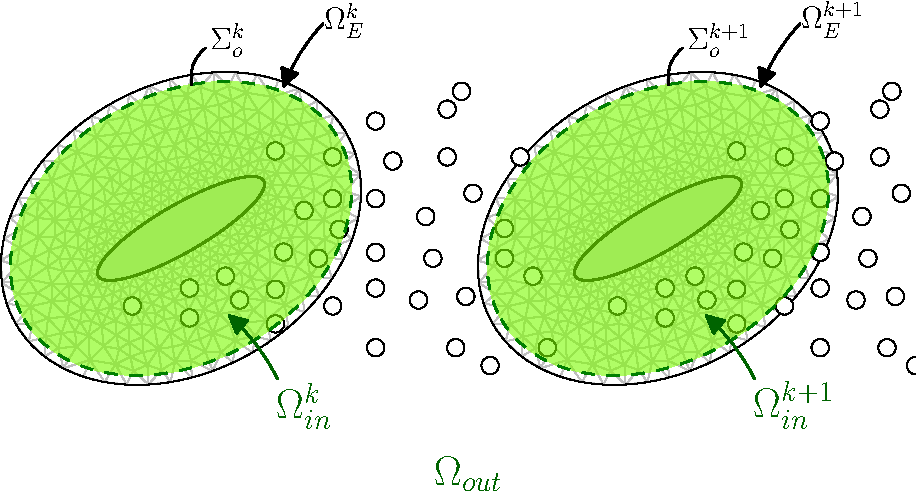
\includegraphics[width=0.9\linewidth]{./figures/coupling/modifiedDomain/domainDecomposition_correctionDomains-crop.pdf}
		\caption{The segregation of the Lagrangian domain $\Omega_L=\Omega_{in}\cup\Omega_{out}$ into the region which is uncorrected $\Omega_{out}$ and the region which is corrected $\Omega_{in} = \bigcup_{k=1}^{N_E}\Omega_{in}^k$.}
		\label{fig:domainDecomposition_correctionDomains}
		\end{figure}				
				
	\subsection{Conservation of Total Circulation}
	\label{subsec:coupling-cotc}
	
	In section \ref{subsec:coupling-vpri} we observed that the method used to determine the strength of particles inside the interpolation domain $\Omega_{I}$ (Figure \ref{fig:domainDecomposition_correctionDomains}) is not accurate for transferring the Eulerian solution to the Lagrangian domain. This approach is erroneous and has a detrimental effect on the total circulation of the Lagrangian domain $\Omega_L$. To ensure that circulation is conserved during the correction step, we to perform an additional correction to the transfer. 
	
	The Lagrangian domain $\Omega_L$ can be divided into two section (as shown in Figure \ref{fig:domainDecomposition_correctionDomains}): 
		\begin{itemize}
		\item Correction region $\Omega_{in}$: The Lagrangian region where the correction takes place: $\Omega_{in} = \bigcup_{k=1}^{N_E}{\Omega_{in}^k}$, where the $k^{\mathrm{th}}$ correction region is defined by $\partial\Omega_{in}^k = \Sigma_{o}^k$, the outer boundary of the interpolation region $\Omega_I^k$.
		\item Unmodified region $\Omega_{out}$: The Lagrangian region that is outside the correction region and is therefore unmodified during the correction step: $\Omega_{out} = \Omega_L\backslash\Omega_{in}$.
		\end{itemize}
	
	The total circulation in the Lagrangian domain before the correction is given as,
		\begin{equation}
		\Gamma^L = \Gamma_{in}^L + \Gamma_{out}^L,
		\label{eq:couping-uncorrected}
		\end{equation}
	where $\Gamma_{in}^L = \sum_k \Gamma_{in}^{L,k}$ is circulation inside $\Omega_{in}$ before they are corrected, and $\Gamma_{out}^L$ is the circulation in $\Omega_{out}$. During the Lagrangian correction step, the circulation $\Gamma_{in}^L$ is corrected and replaced with the corrected circulation $\tilde{\Gamma}_{in}^L$ determine from the Eulerian method, equation \ref{eq:coupling-equalitil2}, resulting in a new total Lagrangian circulation $\tilde{\Gamma}^{L}$ given by,
		\begin{equation}
		\tilde{\Gamma}^{L} = \tilde{\Gamma}_{in}^L + \Gamma_{out}^L,
		\label{eq:coupling-totalLC}
		\end{equation}
	To ensure that the circulation is conserved during the correction step, we required $\Delta \Gamma=0$. This gives us the requirement that,
		\begin{equation}
		\Gamma^{L} = \tilde{\Gamma}^{L}.
		\label{eq:coupling-conserveEq}
		\end{equation}
	or, substituting equation \ref{eq:couping-uncorrected} and equation \ref{eq:coupling-totalLC} into equation \ref{eq:coupling-conserveEq} gives us the requirement that,
		\begin{equation}
		\Gamma_{in}^L = \tilde{\Gamma}_{in}^L, 
		\label{eq:coupling-conserEq2}
		\end{equation}
	and equivalently,
			\begin{equation}
			\Gamma_{in}^{L,k} = \tilde{\Gamma}_{in}^{L,k}.
			\label{eq:coupling-conserEq3}
			\end{equation}		
	This means that the circulation inside the correction region $\Omega_{in}^k$ before the correction should match the circulation after the correction. However, as there exists a slight error in the particle initialization, we introduce a small error in circulation $\epsilon^k$ during the transfer, resulting in,
		\begin{equation}
		\hat{\Gamma}_{in}^{L,k} = \tilde{\Gamma}_{in}^{L,k} + \epsilon_{in}^{L,k},
		\label{eq:coupling-circError}
		\end{equation}
	where $\hat{\Gamma}_{in}^{L,k}$ is the erroneous circulation that was actually transfered and $\tilde{\Gamma}_{in}^{L,k}$ is the correct circulation that was supposed to be transferred. Substituting equation \ref{eq:coupling-circError} into equation \ref{eq:coupling-conserEq2}, we see that the error $\epsilon_{in}^{L,k}$ is written as,
		\begin{equation}
		\epsilon_{in}^{L,k} = \hat{\Gamma}_{in}^{L,k} - \Gamma_{in}^{L,k}.
		\label{eq:coupling-eq22}
		\end{equation}
	and is simply the mismatch in the circulation during the correction step. This error can by modifying the new set of initialized particles in the interpolation domain $\Omega_I$. Using equation \ref{eq:coupling-sumparticlestrengths}, the final strengths of the particles $\tilde{\alpha}_p^k$ for particles $\mathbf{x}_p^k \in \Omega_{in}^k$ is given as,
		\begin{equation}
		\tilde{\alpha}_p^k = \alpha_p^k - \frac{\epsilon_{in}^{L,k}}{N},
		\label{eq:coupling-particlestrengths}
		\end{equation}
	where $\alpha_p^k$ is the uncorrected strengths determined using the local particle area and local vorticity, equation \ref{eq:coupling-standardInitialization}, and $N$ is number of particles inside the correction region $\Omega_{in}^k$. Following this procedure in addition to Stocks Lagrangian correction strategy described in section \ref{subsec:hybrid-lcs}, we will ensure that our hybrid scheme conserves circulation.
	

%	
%	. To satisfy equation ??, we must negate this error, and therefore the true corrected circulation in $\Omega_{in}$ is defined as,
%		\begin{equation}
%		\hat{\Gamma_{\Omega_L}}
%		\end{equation}
%		
%	Investigation the correction strategy of Stock ?? we determine conservation of total circulation is not explicitly ensured.
%	
%	we need to perform additional steps to ensure that the hybrid scheme ensures conservation of total circulation.
%
%	However, we will still have $\epsilon>0$. The mismatch in the interpolated vorticity $\hat{\omega}|_L$ and the vorticity field solution of the Eulerian method $\omega|_E$, will resulting in a loss of total circulation during the correction process. To describe the methodology for correcting the loss in total circulation, let us look at an example unbounded problem (with solid bodies). To generalize the approach, we will investigate a hybrid setup with multiple Eulerian subdomains, Figure ??. 
%	
%	Let $k=\{1,...,N_E\}$, the indices of the Eulerian subdomains $\{\Omega_E^1,...,\Omega_E^k,...\Omega_E^{N_E}\}\subset\Omega_L$ with the total number of Eulerian subdomains $N_E$. Each Eulerian domain $\Omega_E^k$ has its own interpolation domain $\Omega_I^k\subset\Omega_E^k$, where the Lagrangian solution is modified using the Eulerian solutions. The Lagrangian domain therefore can be divided into unmodified $\Omega_{out}$, and modified region $\Omega_{in}$:
%	\begin{itemize}
%	\item Modified region $\Omega_{in}$: The Lagrangian region that is inside the interpolation domains and is modified during the correction step: $\Omega_{in} = \bigcup_{k=}^{N_E}{\Omega_{in}^k}$, where $\Omega_{in}^k=\Omega_L\cap\Omega_{I}^k$, as shown in Figure ??.
%	\item Unmodified region $\Omega_{in}$: The Lagrangian region that is outside the correction region and is therefore unmodified during the correction step: $\Omega_{out} = \Omega_L\backslash\Omega_{in}$, shown in Figure ??.
%	\end{itemize}
%
%	
%
%	
%	To ensure conservation of circulation, the Lagrangian method should satisfy the Kelvin's circulation theorem, $\mathrm{d}\Gamma/\mathrm{d}t=0$. If we assume that the initial total circulation in the Lagrangian method is $\Gamma_{t=0}=0$, then the total circulation in the Lagrangian domain at all times $t$ should be,
%		\begin{equation}
%		\Gamma_{\Omega_{in}}|_L + \Gamma_{\Omega_{out}}|_L = 0.
%		\end{equation}
%
%	The Lagrangian correction steps replaces the Lagrangian circulation inside the correction region $\Gamma_{\Omega_{in}^k}|_L$ with Eulerian circulation $\Gamma_{\Omega_{I}^k}|_E$. But due to the error in interpolation from the Eulerian method to the Lagrangian method, we will have that, 
%		\begin{equation}
%		\Gamma_{\Omega_{I}}|_E + \Gamma_{\Omega_{out}}|_L = \epsilon_{\Gamma},
%		\end{equation}
%	
%	where $\epsilon_{\Gamma}$ is the error in total circulation due to the correction. To negate this error, we will have to modify the strengths of blobs, ensuring conservation of total circulation,
%			\begin{equation}
%			\hat{\alpha}_i = \alpha_i - \frac{\epsilon_{\Gamma}}{N}
%			\end{equation}
%	
%	where $\hat{alpha}_i$ is the corrected particle strength, $\alpha_i$ is determined from Equation ??, and $N$ is the number of particles $\mathbf{x}_i\in\Omega_I$.		
%
%
%	



	%	In equation ??, if $\epsilon=0$, then have that $\Gamma_{\Omega_{in}}|_E = \Gamma_{\Omega_{in}}|_L$. However, due to error in initialization $\epsilon\not0$, at every Lagrangian correction step, there will be a loss in total circulation $\epsilon_{\Gamma}$, where
	%		\begin{equation}
	%		\epsilon_{\Gamma} = \Gamma_{\Omega_{in}}|_E - \Gamma_{\Omega_{in}}|_L
	%		\end{equation}
	%
	%	Following the Kutta's circulation theorem, we require that the total circulation of the Lagrangian method is conserved at all times $\mathrm{d}\Gamma/\mathrm{d}t=0$. Taking $\Gamma_{t=0}=0$, we have that $\Gamma_L=0$ at all times. 
	%	
	%	To compensate this mismatch, by distributing the error uniformly to all the corrected vortex blobs,



	

%	vorticity field $\omega^h$ is represented by a $N$ linear combination of kernel $\delta$ carrying the strengths $\alpha_i$,
%	
%		\begin{equation}
%		\omega \approx \omega^h(\mathbf{x}_j) = \sum_{i=1}^N \alpha_i \delta(\mathbf{x}_j - \mathbf{x_i}).
%		\end{equation}
%	
%	 The standard approach, used by Stock ?? as well, for initializing the particles using the local particle area $h^2$ and the local vorticity $\omega_i$,
%		\begin{equation}
%		\alpha_i = \omega_i\cdot{h^2},
%		\end{equation}
%	where $i$ corresponds to the vortex blobs $\mathbf{x}_i \in \Omega_{int}$.
%	
%	
%
%	
%	The discrete vorticity field $\omega^h$ is represented by a $N$ linear combination of kernel $\delta$ carrying the strengths $\alpha_i$,
%	
%		\begin{equation}
%		\omega \approx \omega^h(\mathbf{x}_j) = \sum_{i=1}^N \alpha_i \delta(\mathbf{x}_j - \mathbf{x_i}).
%		\end{equation}
%	
%	where $\alpha_i$ is the strength of the particle $\mathbf{x}_i\in\Omega_L$. From section ??, the singularity of the kernel $\delta$ can removed by using a Gaussian kernel $\zeta_{\sigma}$, ensuring smooth continuous vorticity field,
%
%	
%	
%	The use of Gaussian kernels introduces additional error in the vorticity field known as the \textit{smoothing error}. In section ??, we investigated significance of the error on the accuracy of the mollified vorticity field.
%	The resulting error $\epsilon$ of this mollified vorticity field $\hat{\omega}$ to the exact vorticity field $\omega$ is:
%			\begin{equation}
%			\epsilon = \epsilon_{\sigma} + \epsilon_h,
%			\label{eq:coupling-totalError}
%			\end{equation}
%			
%	the sum of the smoothing error $\epsilon_{\sigma}$ and the discretization error $\epsilon_h$. Barba and Rossi ??,  			
%		
%	Stock ?? assigned the strength $\alpha_i$ of the particles $x_i\in\Omega_I\subset\Omega_I$ using the standard initialization approach used in vortex methods. The standard initialization uses the local particle area $h^2$ and vorticity from the Eulerian domain $\omega^E$ at the particle $i$, such that:
%		\begin{equation}
%		\alpha_i = \omega_i|_L\cdot{h^2}, \qquad x_i \in \Omega_I.
%		\end{equation}	


%	 In section ??, we observed that when using this approach for a Gaussian kernel results in a mollification of the original intended vorticity distribution $\omega$. The Lagrangian solution of the vorticity field $\omega^L$ is discretized using $N$ vortex particles,
%		 \begin{equation}
%		 \omega |_L \approx \omega^h(\mathbf{x}_j) = \sum_{i=1}^N \alpha_i \delta(\mathbf{x}_j - \mathbf{x_i}).
%		 \end{equation}
%		 
%	 If we use the solution of the Eulerian method $\omega^E$ to initialize the vorticity in the Lagrangian method, the resulting mollified vorticity field is:
%	 
%	  	\begin{equation}
%	 	\omega^E \approx \hat{\omega}^L(\mathbf{x}) = \sum_{i=1}^{N} \alpha_i \zeta_{\sigma}(\mathbf{x} - \mathbf{x}_i).
%	 	\label{eq:coupling-mollifiedVorticityDistributionEquation}
%	 	\end{equation}
%	 
%	 where the mollified vorticity
%	 
%	  Barba and Rossi ??, described this phenomena as a Gaussian blurring of the original vorticity field due to the initialization, due to the \textit{smoothing error} of the Gaussian kernel.
%	 
%	 Figure ?? demonstrates this effect on initializing an example Gaussian vorticity distribution. For a non-decomposed domain initialization, this initialization only has an effect on the distribution of the vorticity field, but conserves the total circulation.
%	 
%	 However, in conjuction with a domain decomposed initialization, 
%	 The results 
	


\section{Modified Lagrangian Correction Algorithm}
\label{sec:coupling-mlca}


	In this section we will investigate the algorithm used for the \textit{Correct Lagrangian} step of our hybrid evolution, Figure \ref{fig:flowchart_simpleCoupling_correction}. We first summarized the algorithm used by Stock \cite{Stock2010a} in section \ref{subsec:hybrid-lcs}. However in section \ref{seec:coupling-mthlcs}, we determine that the algorithm required some modification to ensure minimum interpolation error and conservation of total circulation. Therefore, we will also describe the algorithm required to implement these modifications.
	
		\begin{figure}[H]
			\centering
			\begin{tikzpicture}
				[node distance=.8cm, start chain=going below,]
				\node[punktchainS, join] (correct) {\textsf{\textbf{Correct Lagrangian}}};
			    \node[punktchainO, join] (evolveL) {\textsf{Evolve Lagrangian}};
			    \node[punktchainO, join] (bcE)     {\textsf{Determine Eulerian \\boundary conditions}};
			    \node[punktchainO, join] (evolveE) {\textsf{Evolve Eulerian}};
			\end{tikzpicture}
			\caption{Flowchart of the hybrid evolution, focusing on the $1^{\mathrm{st}}$ step: Correct the Lagrangian solution.}
			\label{fig:flowchart_simpleCoupling_correction}
		\end{figure}
		
	The general approach we used to perform transfer of the solution from the Eulerian to Lagrangian domain is by substituting particles inside the zone of correction (i.e the correction region $\Omega_{in}$ as shown in Figure \ref{fig:domainDecomposition_kthDomain}) with a correct set of particles that represent the more accurate Eulerian solution. We need to determine the vorticity at their positions so that we can use equation \ref{eq:coupling-standardInitialization} to initialize the strengths of these new particles. The vorticity at these positions can be determined by interpolating the Eulerian solution onto their positions. 
	
	However, determining the location of the particle w.r.t the unstructured grid of the Eulerian method is computationally expensive. Therefore, we will first interpolate the Eulerian solution onto a regular grid. Performing a search algorithm on such grid is computationally less expensive. Furthermore, to ensure that the interpolation of vorticity from unstructured grid onto a regular structured grid is also efficient, the regular structured grid will be bounded to the Eulerian domain. In such case, the interpolation problem only needs to be setup once as the transfer weights remains unchanged throughout the simulation. 
	
	The final stages of the Lagrangian correction step is to ensure that the total circulation is conserved. We will therefore determine the strength of the vortex sheet and the total strength of the newly generated vortex blobs such that circulation is conserved.
	
	The algorithm describing these procedure is organized and summarized as follows:
	\begin{enumerate}
	\item \textbf{Interpolate vorticity}: Interpolate the vorticity from the unstructured Eulerian mesh onto a structured grid that is bounded to the Eulerian domain $\Omega_E$.
	\item \textbf{Remove particles}: Remove particles that are inside the interpolation domain $\Omega_{I}$.
	\item \textbf{Generate particles}: Generate zero-strength particle inside the interpolation domain $\Omega_{I}$.
	\item \textbf{Assign strengths to particles}: Interpolate the vorticity from the structured grid onto the position of the newly generated particles. Using the standard particle initialization approach described in section \ref{subsec:coupling-vpri}, assign the strengths to the newly generated particles. 
	\item \textbf{Correct total circulation}: Using the approach described in section \ref{subsec:coupling-covs} and section \ref{subsec:coupling-cotc}, determine the total strength of the vortex sheet and total strength of the newly generated vortex blobs such that the total circulation is conserved.
	\end{enumerate}
	
	The steps 1 to 4 will be described for the $k^{\mathrm{th}}$ Eulerian domain $\Omega_E^k$. These steps simply needed to be iterated for all $N_E$ number of Eulerian domains (i.e bodies) in the case of a multi-body problem. The last step of correcting the total circulation is performed for all the Eulerian domains simultaneously as we require the knowledge of total circulation. A detailed description of the each steps of the Lagrangian correction algorithm is given below.
	
	
	% Summary of the algorithm
	% Algorithm to the coupled evolution of the hybrid method.
	% Refer to chapters
	% Flow charts.
	% Refer to the code
	% Proposed modifications
	
	\subsection{Interpolate Vorticity}
	\label{subsec:coupling-iv}
	In this step, we will interpolate the vorticity from the unstructured grid of the Finite Element method onto a regular structured grid, that is bounded to the Eulerian domain $\Omega_E^k$. The algorithm for interpolating the vorticity from the unstructured grid onto a structured grid is as follows:

		\begin{figure}[!b]
	     \centering
	     \begin{subfigure}[t]{0.45\textwidth}
	             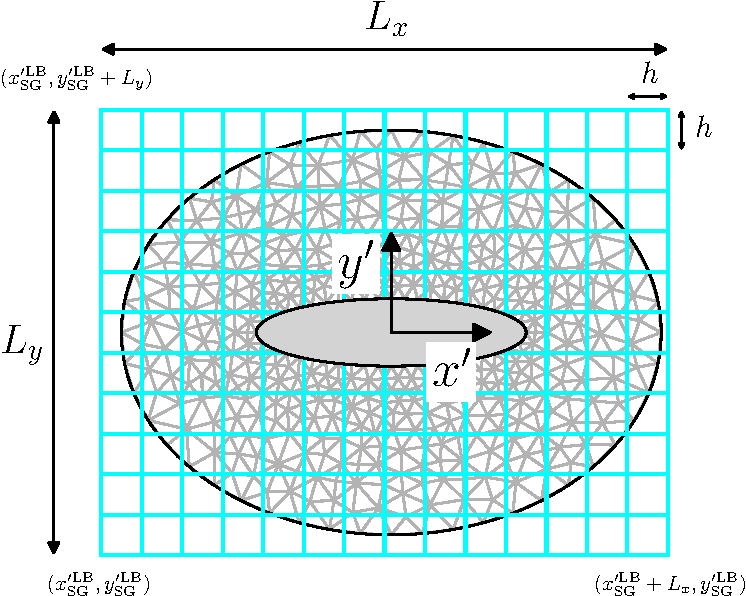
\includegraphics[width=\textwidth]{./figures/coupling/interpolateVorticity/structuredGrid_localCoord-crop.pdf}
	             \caption{Local coordinate system}
	             \label{fig:structuredGrid_localCoord}
	     \end{subfigure}%
	     ~ %add desired spacing between images, e. g. ~, \quad, \qquad etc.
	       %(or a blank line to force the subfigure onto a new line)
	     \begin{subfigure}[t]{0.45\textwidth}
	             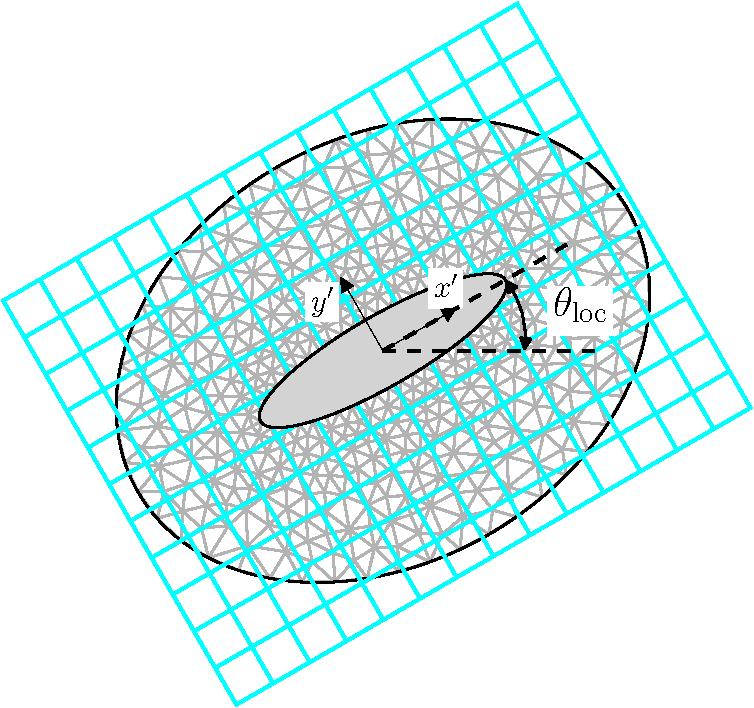
\includegraphics[width=0.9\textwidth]{./figures/coupling/interpolateVorticity/structuredGrid_globCoor-crop.pdf}
	             \caption{Global coordinate system}
	             \label{fig:structuredGrid_globCoor}
	     \end{subfigure}
	     
	     \caption{Structured grid ({\color{plotCyan}{\textbf{cyan}}}) covering the entire Eulerian grid (\textbf{black}).}
	     \label{fig:structuredGrid_Def}
		\end{figure}

	\begin{enumerate}[label=1.\alph*)]
	\item \textbf{Setup a structured grid} (\textit{only once}): A \printAcron{structured grid}{SG} is created in the local coordinate system of the $k^{\mathrm{th}}$ Eulerian domain $\Omega_E^k$. The grid is constructed such that it covers the \printAcron{Eulerian grid}{SG} of the Eulerian method, as shown in Figure \ref{fig:structuredGrid_localCoord}.

	The parameters that define the structured grid in the local coordinate system are the starting point of the grid (the left-bottom corner) $(x_{\mathrm{SG}}'^{\mathrm{LB}}, y_{\mathrm{SG}}'^{\mathrm{LB}})$, the horizontal length of the grid $L_x$, the vertical length of the grid $L_y$, and the grid cell spacing $h$ (which is equal to the nominal blob spacing). The lengths $L_x$ and $L_y$ are defined such that it is a multiple of the grid spacing $h$,
		\begin{subequations}
		\begin{align}
		L_x &= n_x \cdot h\\
		L_y &= n_y \cdot h,
		\end{align}
		\label{eq:structureGridLengths}
		\end{subequations}
	where $n_x$ and $n_y$ are the number of cells in the horizontal and the vertical direction, respectively. The transformation of the structured grid follows that of the body and therefore the structure grid does not move w.r.t to the Eulerian grid.  For more details on the transformation from the local coordinate system to the global, see appendix \ref{app:coordinateSystems}. Figure \ref{fig:structuredGrid_globCoor} shows the structured grid bounded to the body in the global coordinate system.
	
	%In the local coordinate system, the SG starts from the left bottom corner $(x_{\mathrm{SG}}'^{\mathrm{LB}}, y_{\mathrm{SG}}'^{\mathrm{LB}})$ and extends by $L_x$ and $L_y$ in the $x$ and the $y$ direction respectively, as shown in Figure \ref{fig:structuredGrid_localCoord}. The SG cells are square with the sides having the length $h$, the nominal blob spacing. In the global coordinate system, the structure grid is transformed with the same local rotational angle $\theta_{loc}$ as the EG, according to the transformation described in appendix \todo{??}.
	\begin{figure}[!b]
		\centering
		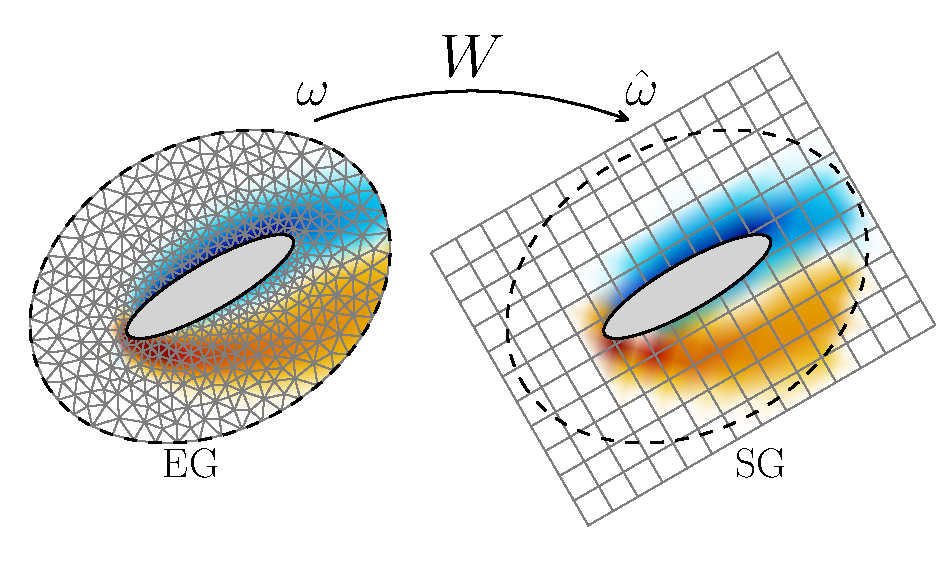
\includegraphics[width=0.9\linewidth]{./figures/coupling/interpolateVorticity/interpolation_EG2SG-crop.pdf}
		\caption{Interpolation of the vorticity $\omega$ from the Eulerian grid onto the structured grid using equation \ref{eq:coupling-interpolationeq2}.}
		\label{fig:interpolation_EG2SG}
		\end{figure}		
	
	
	\item \textbf{Determine the weights} (\textit{only once}): The interpolation of the Eulerian vorticity $\omega$ from the Eulerian grid onto the structured grid is represented as,
		\begin{eqnarray}
		\hat{\omega}_j = \sum_i \omega_i W_{ij},
		\label{eq:coupling-interpolationeq2}
		\end{eqnarray}
	where $\hat{\omega}_j$ is the interpolated vorticity on the structured grid and $W$ is the interpolation weights. As the structured grid is bounded to the Eulerian grid, the weights of the interpolation does not change throughout the simulation and only needs to be calculated once. This makes the interpolation problem computationally very efficient.
	
	\item \textbf{Interpolate the vorticity}: This step needs to be perform at every Lagrangian correction step. The vorticity $\hat{\omega}$ on the structured grid is calculated by simply solving the pre-assembled problem, defined by equation \ref{eq:coupling-interpolationeq2}. 
	\end{enumerate}


	To construct the interpolation problem, we used a tree search algorithm from the CGAL library \cite{CGAL}, included in \fenics and adapted for fast repeated evaluation by Mortenson (Fenicstools \cite{fenicstools}). The algorithm probes the vorticity function $\omega$ of the unstructured Eulerian grid at the nodes of the structured grid $(x_{\mathrm{SG}}, y_{\mathrm{SG}})$. Figure \ref{fig:interpolation_EG2SG} shows a depicts the result of the transferring the vorticity from the unstructured grid to the structured grid. The vorticity on the structured grid can then be efficiently interpolated onto the positions of the particles. %This is performed using an efficient index search algorithm to find the location of particles in the SG, section \ref{subsec:coupling-as}. If we had not employed this approach and instead directly transfered the vorticity from the unstructured EG onto the vortex blobs $\mathbf{x}_i$, we would require a computationally expensive search algorithm to determine the position of each blob w.r.t to the nodes of the unstructured grid $(x_{\mathrm{EG}}, y_{\mathrm{EG}})$. This would require a construction of the interpolation matrix at each iteration, drastically reducing the efficiency of interpolation.
		
		
		
	\subsection{Remove Particles}
	In this step, the uncorrected vortex particles inside the correction region $\Omega_{in}$ (as shown in Figure \ref{fig:domainDecomposition_correctionDomains}) will be removed. Let $\mathcal{P}$ be the set of particle indices with position $\mathbf{x}_p\in\Omega_L$. The algorithm for removing the particles $p$ is as follows:
	
	\begin{figure}[p]
     \centering
     \begin{subfigure}[t]{0.55\textwidth}
		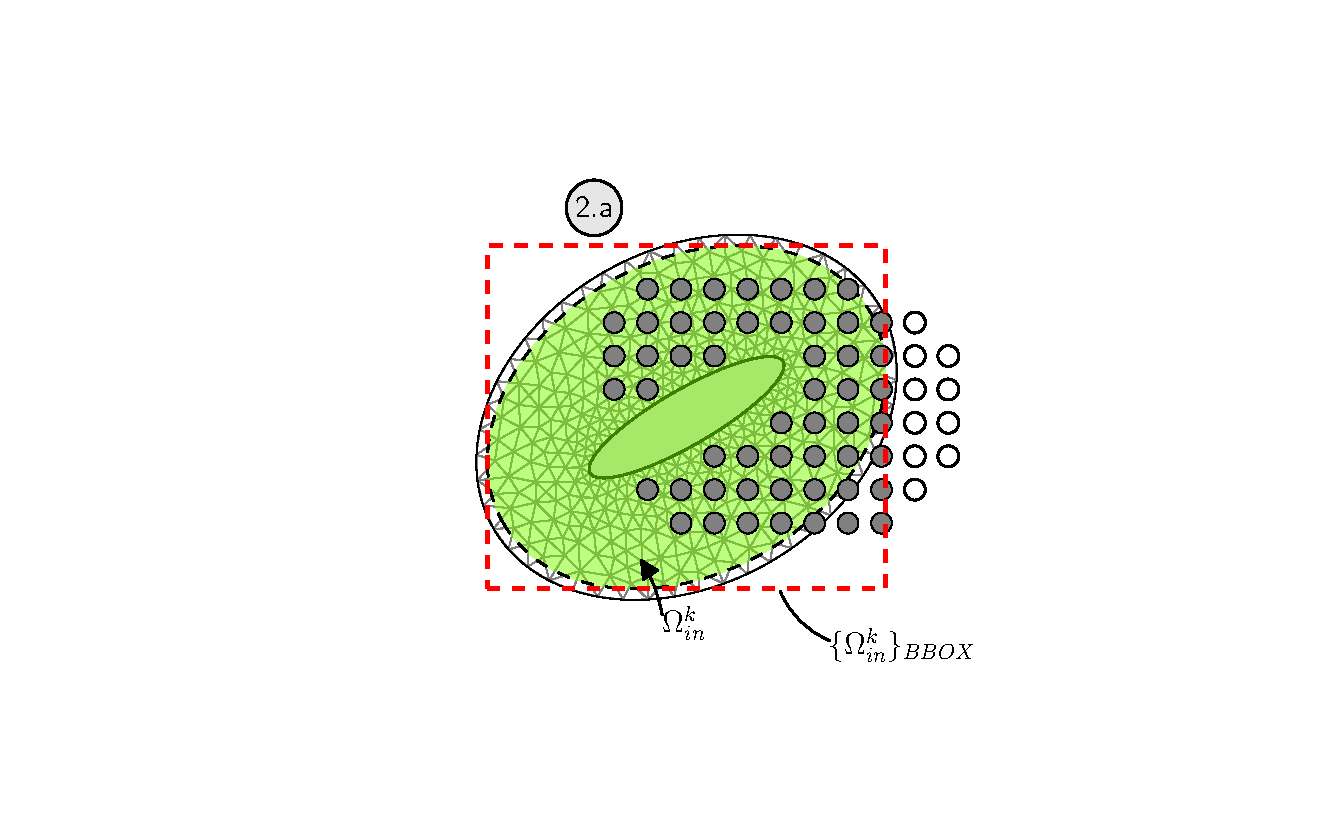
\includegraphics[trim=8.05cm 2.85cm 5.4cm 3.05cm, clip, width=0.9\linewidth]{./figures/coupling/removeParticles/removeParticles_part1.pdf}
		\caption{Step 2.a: Find the particles inside the BBOX of $\Omega_{in}^k$}
		\label{fig:removeParticles_part1}
	 \end{subfigure}%
	 \quad%3.84cm
     \begin{subfigure}[t]{0.55\textwidth}
		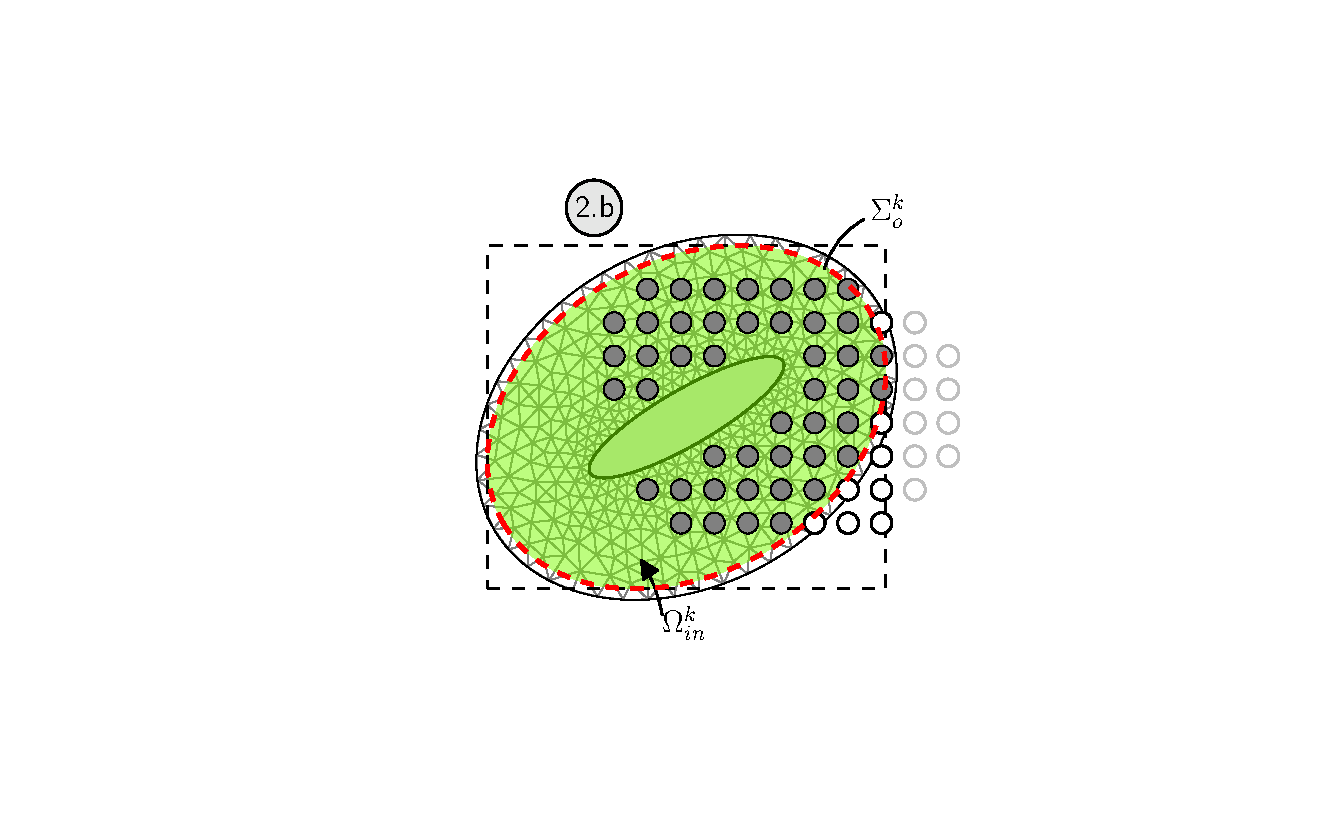
\includegraphics[trim=8.05cm 2.85cm 5.4cm 3.05cm, clip, width=0.9\linewidth]{./figures/coupling/removeParticles/removeParticles_part2.pdf}
		\caption{Step 2.b: Among them, find the particles that are also inside the correction region $\Omega_{in}^k$}
		\label{fig:removeParticles_part2}
	 \end{subfigure}%	 
	 \quad
     \begin{subfigure}[t]{0.55\textwidth}
		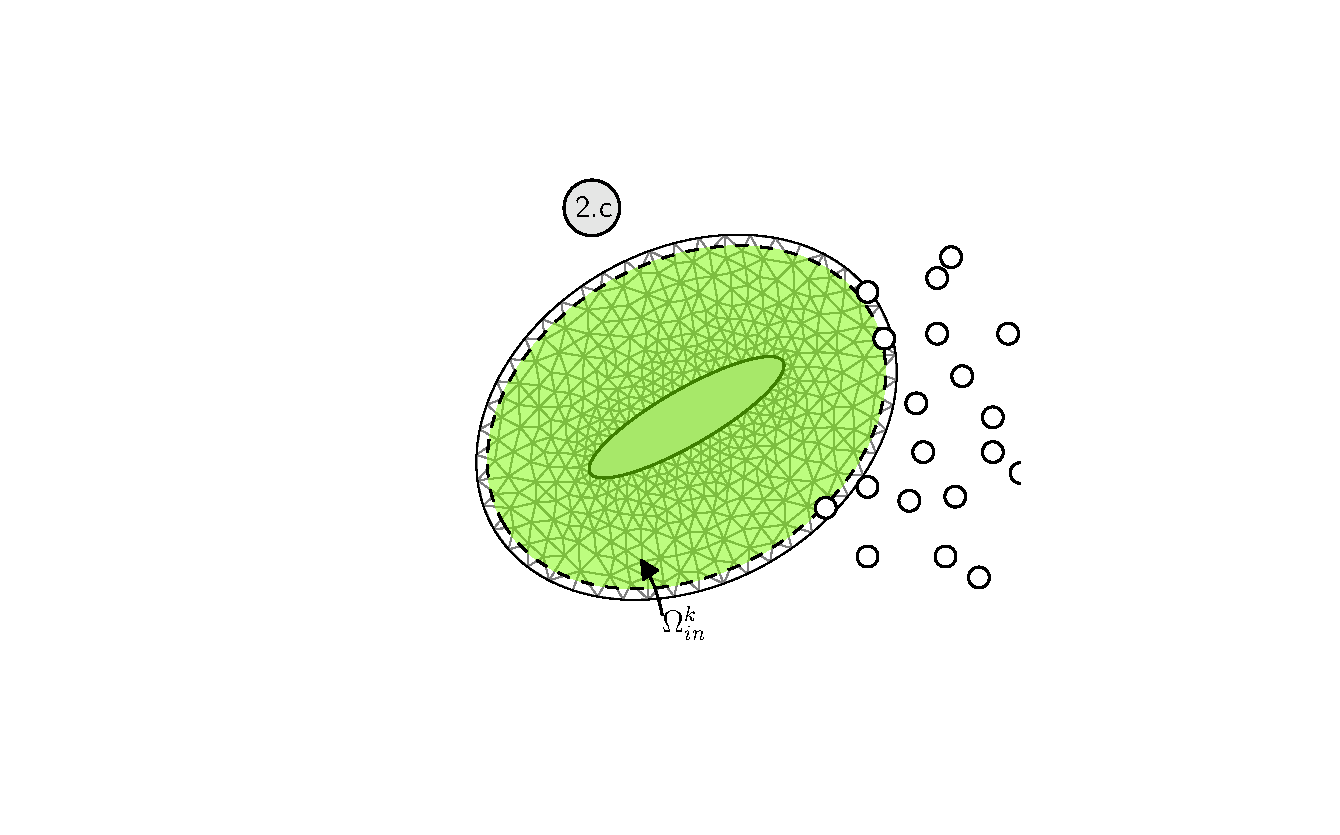
\includegraphics[trim=8.05cm 2.85cm 5.4cm 3.05cm, clip, width=0.9\linewidth]{./figures/coupling/removeParticles/removeParticles_part3.pdf}
		\caption{Step 2.c: Remove the particles that are inside the correction region $\Omega_{in}^k$}
		\label{fig:removeParticles_part3}
	 \end{subfigure}%		 

     \caption{Figures depicts the computationally optimized algorithm for finding and removing the vortex particles inside the correction region $\Omega_{in}^k$.}
     \label{fig:removeParticles}
	\end{figure}	

	
	\begin{enumerate}[label=2.\alph*)]
	\item \textbf{Find the particles inside the BBOX of $\Omega_{in}^k$}: Find the particles $p$ that lie inside the minimum bounding box of the correction domain $\Omega_{in}^k$. Let $\mathcal{P}_{\mathrm{BBOX}}^k$ be the set of particles indices that are within the bounding box of the correction domain $\Omega_{in}^k$, the gray particles shown in Figure \ref{fig:removeParticles_part1}. The minimum bounding box (shown in red) is constructed using the outer boundary polygon of the correction region $\Sigma_{o}$. Performing this search algorithm is computationally efficient and reduces the number of particles of interest for the more expensive \textit{point-in-polygon} search algorithm of the next step.
	\item \textbf{Find the particles inside the correction region $\Omega_{in}^k$}: Determine which of the particles in the set $\mathcal{P}_{\mathrm{BBOX}}^k$ also lie within the correction domain $\Omega_{in}^k$. Let $\mathcal{P}_{in}^k\subset\mathcal{P}_{\mathrm{BBOX}}^k$ be the set of particles that also lie inside the correct region $\Omega_{in}^k$, the gray particles in Figure \ref{fig:removeParticles_part2}. The search algorithm is performed using a \textit{point-in-polygon} test with the outer boundary $\Sigma_{o}^k$ (shown in red).
	\item \textbf{Remove particles inside correction region}: Remove the set of particles inside the correction region $\mathcal{P}_{in}^k$. These particles have a total circulation of $\Gamma_{in}^{L,k}$ ( as used in Equation \ref{eq:couping-uncorrected}) which needs to be compensated later to ensure conservation of total circulation. Figure \ref{fig:removeParticles_part3} shows the final set of particles after \textit{remove particle} step.
	\end{enumerate}	
		
	To perform the point-in-polygon test, we used the \texttt{pnpoly} function of \texttt{matplotlib}, the python 2D plotting library created by Hunter \cite{Hunter:2007}. The function implemented the \textit{point inclusion in polygon} test algorithm developed by Franklin \cite{franklin2006pnpoly}. The algorithm is based on the crossings test, which determines whether the point is inside the polygon by determining the number of the times a semi-infinite ray originating from the point intersects with the polygon.
	
%	When we have multiple bodies, the \textit{remove particle} step is repeated for each of the $k^{\mathrm{th}}$ correction region $\Omega_{in}^k$.

	
	\subsection{Generate Particles}
	
		\begin{figure}[p]
	     \centering
	     \begin{subfigure}[t]{0.55\textwidth}
			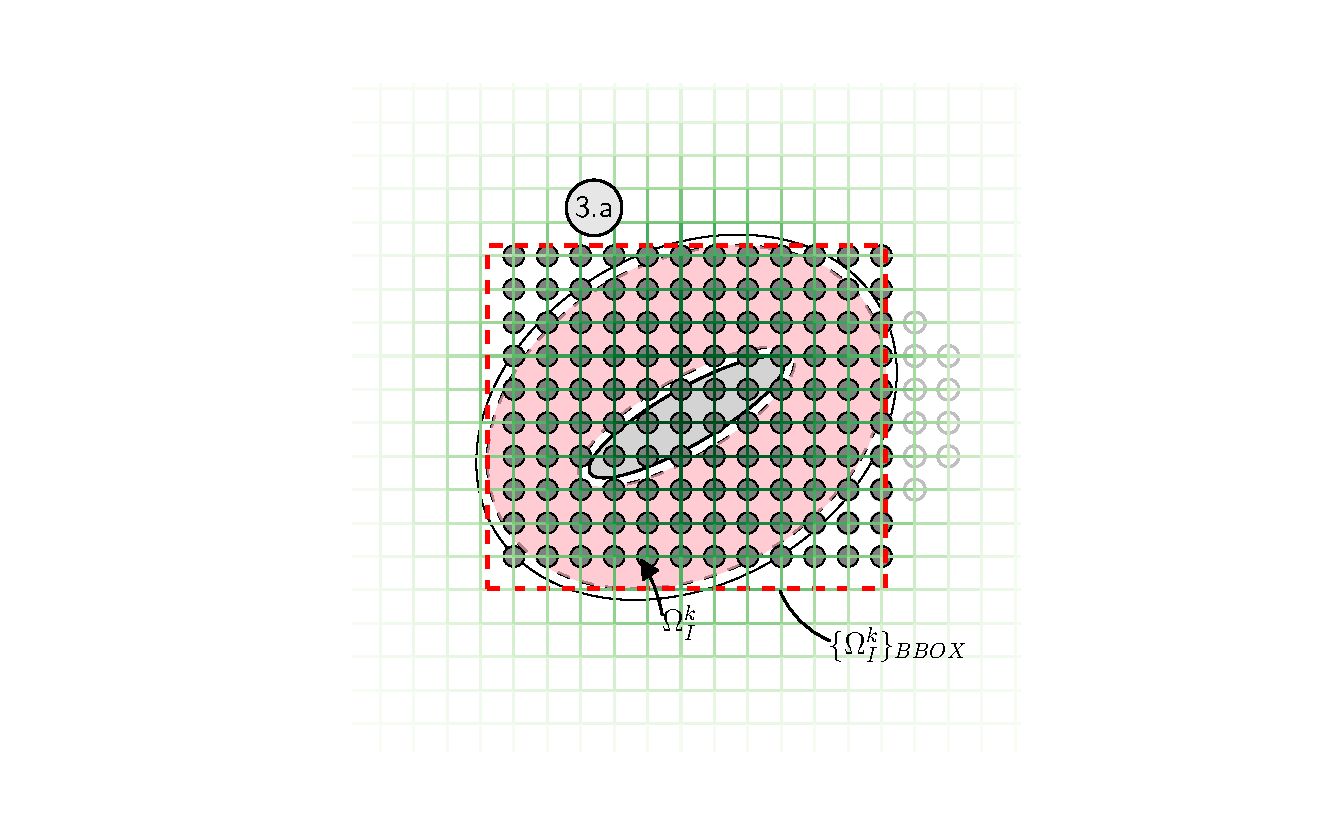
\includegraphics[trim=8.05cm 2.85cm 5.4cm 3.05cm, clip, width=0.9\linewidth]{./figures/coupling/generateParticles/generateParticles_part1.pdf}
			\caption{Step 3.a: Generate particles inside the BBOX of the interpolation domain $\Omega_{I}^k$ matching the Lagrangian mesh}
			\label{fig:generateParticles_part1}
		 \end{subfigure}%
		 \quad %3.84cm
	     \begin{subfigure}[t]{0.55\textwidth}
			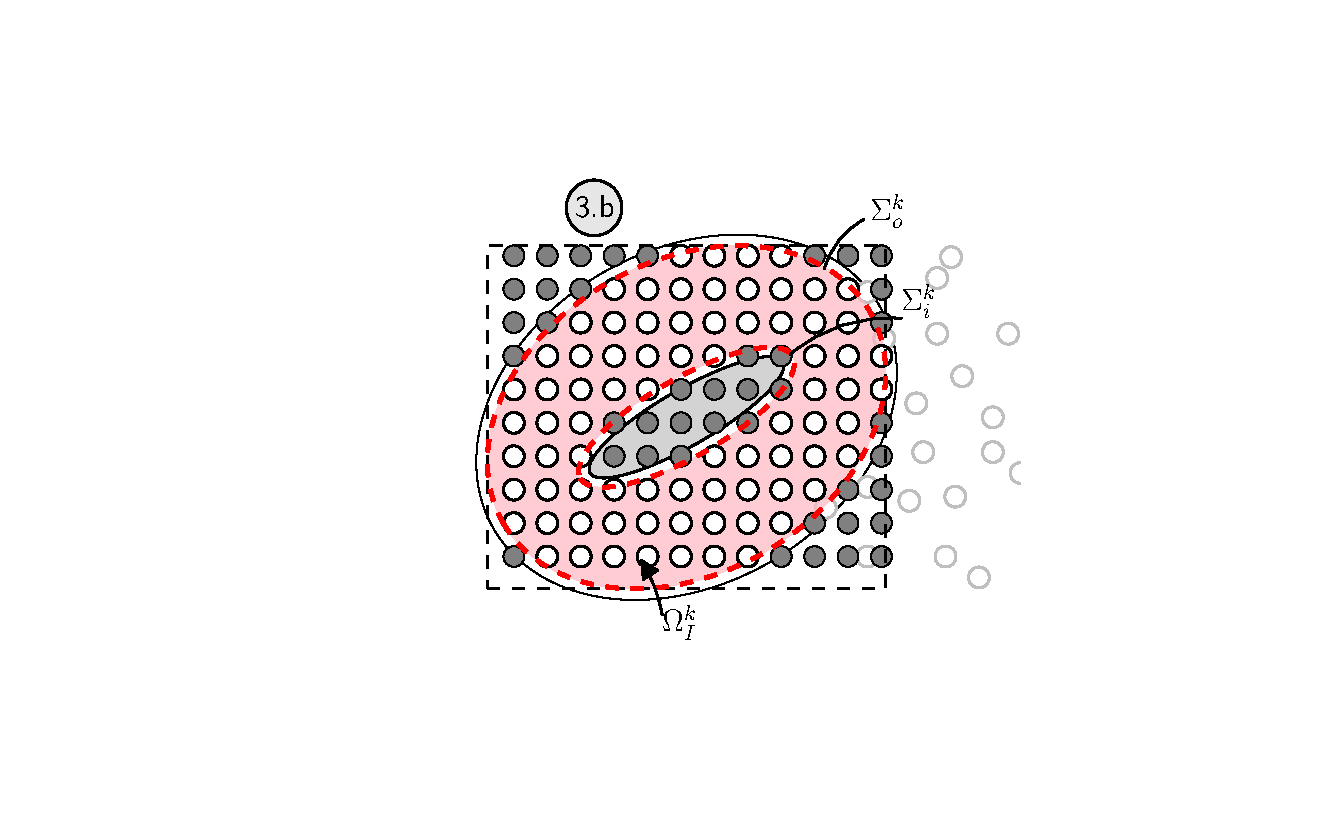
\includegraphics[trim=8.05cm 2.85cm 5.4cm 3.05cm, clip, width=0.9\linewidth]{./figures/coupling/generateParticles/generateParticles_part2.pdf}
			\caption{Step 3.b: Among them, find the particles that are outside the interpolation domain $\Omega_{I}^k$}
			\label{fig:generateParticles_part2}
		 \end{subfigure}%	 
		 \quad
	     \begin{subfigure}[t]{0.55\textwidth}
			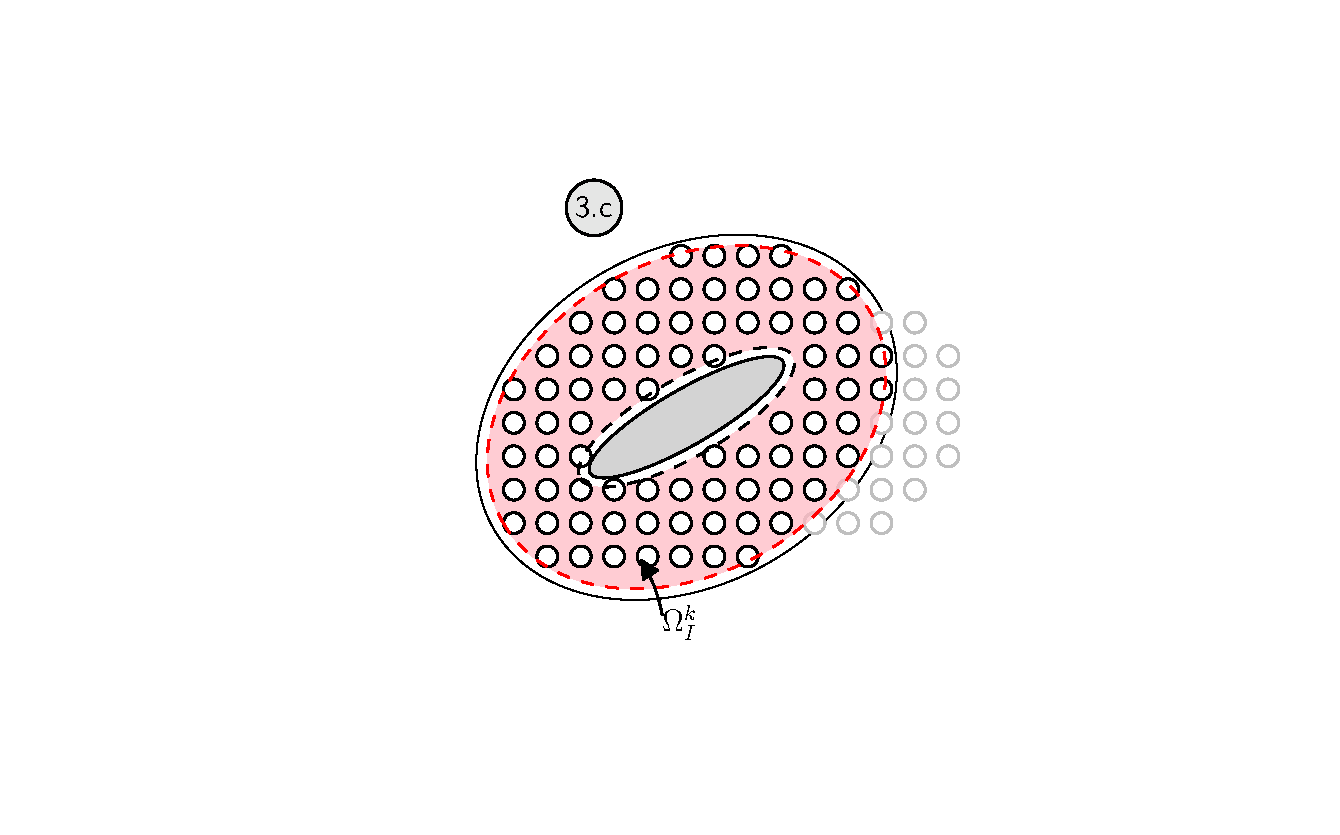
\includegraphics[trim=8.05cm 2.85cm 5.4cm 3.05cm, clip, width=0.9\linewidth]{./figures/coupling/generateParticles/generateParticles_part3.pdf}
			\caption{Step 3.c: Remove the newly generated particles that are outside interpolation domain $\Omega_{I}^k$}
			\label{fig:generateParticles_part3}
		 \end{subfigure}%		 
	
	     \caption{Figures depicts the algorithm for generating vortex particles inside the interpolation domain $\Omega_{I}^k$ matching the Lagrangian mesh.}
	     \label{fig:generateParticles}
		\end{figure}	
	
	In order to interpolate the solution from the Eulerian domain onto Lagrangian domain, we require the knowledge of the particle positions. In this step, we will generate zero-strengths particles inside the interpolation region $\Omega_I^k$ (Figure \ref{fig:domainDecomposition_kthDomain}).
	
	The algorithm for generating zero-strength particles inside the $k^{\mathrm{th}}$ interpolation domain $\Omega_{I}^k$ is as follows:
	\begin{enumerate}[label=3.\alph*)]
	\item \textbf{Generate particles inside the BBOX of interpolation domain $\Omega_I^k$}: Generate zero-strength particles inside the bounding box of the interpolation region $\Omega_{I}^k$, the gray particles shown in Figure \ref{fig:generateParticles_part1}. The particles are positioned at the nodes of the global Lagrangian remeshing grid (introduced in section \ref{subsec:remeshing}) such that particles are equally distributed as satisfies the overlap ratio criteria. Let $\hat{\mathcal{P}}_{\mathrm{BBOX}}^k$ be the set all newly generated particles (gray) inside the bounding box at the nodes of the Lagrangian method (green).
	
	\item \textbf{Find newly generated particles inside interpolation region $\Omega_I^k$}: We perform a point-in-polygon test for the newly generated particles $\hat{\mathcal{P}}_{\mathrm{BBOX}}^k$, so that we can neglect the particles that are outside the interpolation region $\Omega_{I}^k$. Let $\hat{\mathcal{P}}_{in}^k \subset \hat{\mathcal{P}}_{\mathrm{BBOX}}^k$ be the set of particles (white) that are within the interpolation region $\Omega_{I}^k$. Figure \ref{fig:generateParticles_part2} shows the set of particles that are not inside the interpolation region $p_i\notin\hat{\mathcal{P}}_{in}$ (gray).
	
	\item \textbf{Remove all the newly generated particles outside the interpolation region $\Omega_{I}^k$}: Remove all the newly generated particles that outside the interpolation region $p_i \notin \hat{\mathcal{P}}_{in}$. Figure \ref{fig:generateParticles} shows the final distribution of the particles, with a uniformly distributed particles inside the interpolation region $\Omega_I^k$ without any gaps.
	\end{enumerate}
	
	In combination with the \textit{remove particle} step and the \textit{generate particle} step, we can ensure that vortex blobs are uniformly distributed inside the interpolation region $\Omega_I^k$ without any gaps. If the initial distribution of the particles (as shown in Figure \ref{fig:removeParticles_part1}) was not modified, we would see that due to the gaps in particle distribution not all vorticity could be interpolated to the Lagrangian method. However, now with the uniform distribution (as shown in Figure \ref{fig:generateParticles_part3}), this is no longer the case.
	
	
	\subsection{Assign Strengths of Particles}
	\label{subsec:coupling-as}
	
	In this step, we will describe the algorithm for assigning strengths to the newly generated particles based on theory summarized in section \ref{subsec:coupling-vpri}. The strengths of the particle are determined by first interpolating the vorticity from the structured grid onto the position of the newly generated zero-strength vortex blobs, then using equation \ref{eq:coupling-standardInitialization} to assign the strengths.
	
	\begin{figure}[p]
	     \centering
	     \begin{subfigure}[t]{0.55\textwidth}
			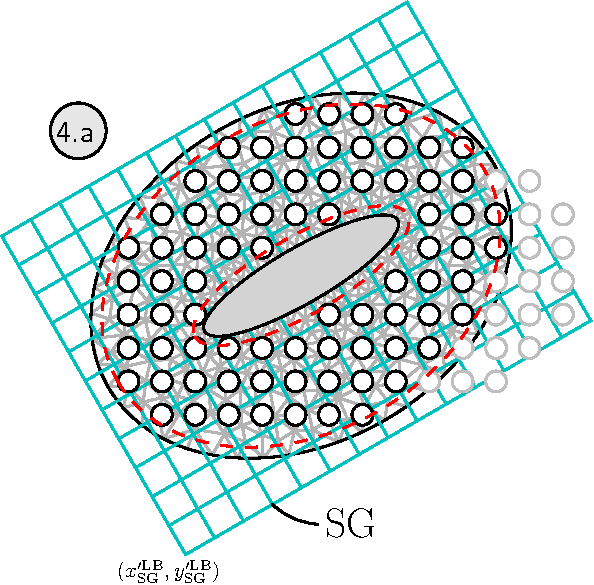
\includegraphics[width=\linewidth]{./figures/coupling/assignStrength/assignStrength_part1-crop.pdf}
			\caption{Step 4.a: Determine the orientation of the SG w.r.t to the newly generated particles}
			\label{fig:assignStrength_part1}
		 \end{subfigure}%
		 \qquad %3.84cm
	     \begin{subfigure}[t]{0.5\textwidth}
			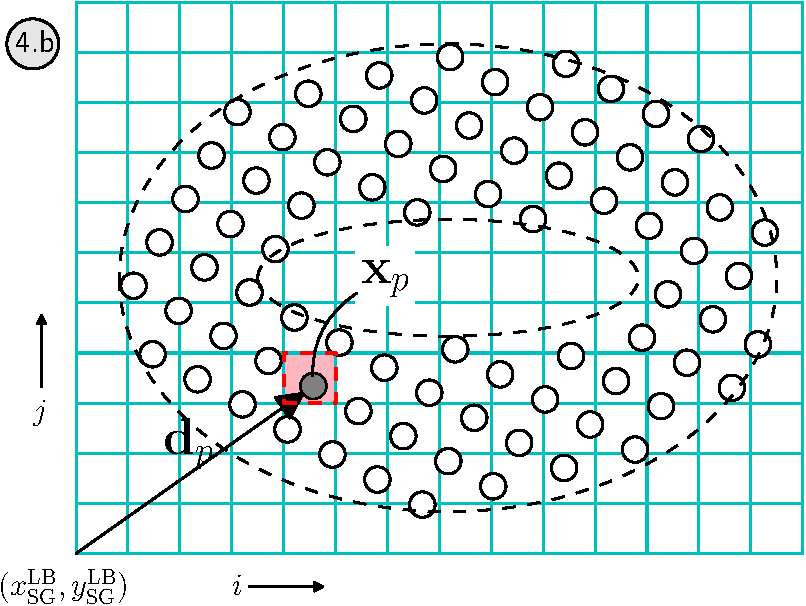
\includegraphics[width=\linewidth]{./figures/coupling/assignStrength/assignStrength_part2-crop.pdf}
			\caption{Step 4.b: Project vortex blobs onto the coordinate system of the SG}
			\label{fig:assignStrength_part2}
		 \end{subfigure}%	 
		 \qquad \qquad \qquad \qquad \qquad
	     \begin{subfigure}[t]{0.4\textwidth}
			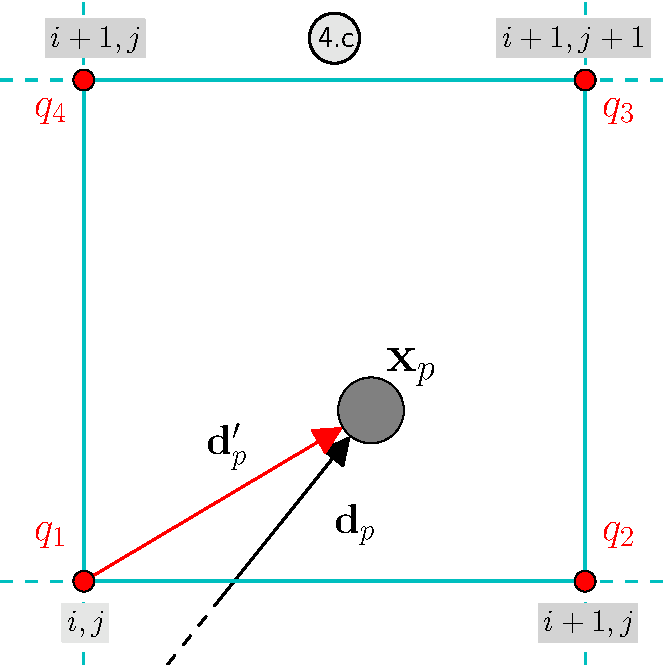
\includegraphics[width=\linewidth]{./figures/coupling/assignStrength/assignStrength_part3-crop.pdf}
			\caption{Step 4.c: Determine the weights of the bilinear interpolation}
			\label{fig:assignStrength_part3}
		 \end{subfigure}%		 
	
	     \caption{Figures depicts the algorithm for assigning the strengths of the vortex particles inside the interpolation domain $\Omega_{I}^k$.}
	     \label{fig:assignStrength}
		\end{figure}		
	
	The algorithm for assigning the strengths of the newly generated particles inside the interpolation domain $\Omega_I^k$ is as follows:
	\begin{enumerate}[label=4.\alph*)]
	\item \textbf{Determine the orientation of the SG w.r.t to the newly generated particles}: The interpolation algorithm starts by first determining the position of the structure grid SG w.r.t to the vortex blobs. The key parameters that define the position and the orientation of the structured grid in the global coordinate system is the position of the left bottom corner $(x_{\mathrm{SG}}^{\mathrm{LB}},y_{\mathrm{SG}}^{\mathrm{LB}})$, and the rotational angle $\theta_{loc}$, as described in section \ref{subsec:coupling-iv}. Figure \ref{fig:assignStrength_part1}, shows the global position of the structured grid w.r.t to the newly generated vortex blobs.
	
	\item \textbf{Project the blobs into the coordinate system of the SG}: Once we know the position of the $SG$, we need to determine in which cells of the SG, the newly generated set of particles $\hat{\mathcal{P}}_{in}^k$ are located. To determine this, we need to project the vortex blobs onto the coordinate system of the structured grid. Figure \ref{fig:assignStrength_part2} shows the projected orientation of the vortex blobs in the local coordinate system of the structured grid. Let $\mathbf{d}_p = |\mathbf{x}_p-\mathbf{x}_{SG}|$ be the offset of the particle $p$ w.r.t to the left bottom corner of the structured grid. In the local coordinate system, the offset $\mathbf{d}_p$ is given by,
		\begin{equation}
		\mathbf{d}_p = 
		\begin{bmatrix}
		d_{x,p}\\
		d_{y,p}\\
		\end{bmatrix} = \begin{bmatrix}
		\cos\theta_{loc} & \sin\theta_{loc}  \\
		-\sin\theta_{loc}  & \cos\theta_{loc} 
		\end{bmatrix} \cdot \begin{bmatrix}
		x_{p}-x_{\mathrm{SG}}^{\mathrm{LB}}\\
		y_{p}-y_{\mathrm{SG}}^{\mathrm{LB}}
		\end{bmatrix}
		\end{equation}
	where $d_{x,p}$ and $d_{y,p}$ are the horizontal and the vertical distance from the left bottom corner, as shown in the Figure \ref{fig:assignStrength_part2}. 
	
	In the local coordinate, the nodes of the structured grid are addressed by index $i$ and $j$ for $x$ and $y$ direction respectively. Let $q_1,q_2,q_3,q_4$ refer to the four nodes of the cell in which the particle $p$ is located, as shown in Figure \ref{fig:assignStrength_part2}). In this cases, the coordinates of these nodes in the local coordinate system are given as,
%	
%	$q_p = \{q_{1,p},q_{2,p},q_{3,p},q_{4,p}\}$ be the four nodes of the cell in which particle $p$ is located, coordinates of the four nodes are given as
%	
%	
%	 as shown in Figure \ref{fig:assignStrength_part2}). Let $T_k$ be the cell (shown in pink) in which the 
%	$k^{\mathrm{th}}$ particle in the set of newly generated $\mathbf{x}_k\in\mathcal{P}_{in}$ reside. The position of the cell, from the left-bottom corner of the grid can be determined by the column index $i$ and the row index $j$. The cell index of $T_k$ can be determined directly from the offset of the particle from the left-bottom corner of the grid $\mathbf{d}_k$, as is given by,
%			\begin{subequations}
%			\begin{align}
%			i_k &= \left\lfloor\frac{d_{x,k}}{h}\right\rfloor\\
%			j_k &= \left\lfloor\frac{d_{y,k}}{h}\right\rfloor,
%			\end{align}
%			\label{eq:floorindex}
%			\end{subequations}
%	where we use the floor function to obtain $i_k\in\{0,1,...,L_x/h\}\subset\mathbb{Z}$ and $j_k\in\{0,1,...,L_y/h\}\subset\mathbb{Z}$ as integers. The cell $T_k$ has four nodes and the coordinates of the nodes are:
			\begin{eqnarray}
			\begin{aligned}
			\mathbf{x}'_1 &= (i_p \cdot h, j_p \cdot h),\\
			\mathbf{x}'_2 &= \left([i_p+1]\cdot h, j_p \cdot h\right),\\
			\mathbf{x}'_3 &= ([i_p+1]\cdot h, [j_p+1] \cdot h),\\
			\mathbf{x}'_4 &= (i_p \cdot h, [j_p+1] \cdot h),\\
			\end{aligned}
			\label{eq:wip}
			\end{eqnarray}
	
	where $i_p$ and $j_p$ are determined by a floor function,
		\begin{subequations}
			\begin{align}
			i_p &= \left\lfloor\frac{d_{x,p}}{h}\right\rfloor\\
			j_p &= \left\lfloor\frac{d_{y,p}}{h}\right\rfloor.
			\end{align}
			\label{eq:floorindex}
		\end{subequations}
	
	\item \textbf{Determine the weights of the bilinear interpolation}: Onces we determine in location of the particle $p$ in terms of index $i_p$ and $j_p$, we can set up a bilinear interpolation problem for transferring the vorticity from the nodes of the structured grid onto the position of the particle. The bilinear interpolation of vorticity is given as,
		\begin{equation}
		\hat{\omega}(\mathbf{x}_p) = \sum_{q=1}^4 W_{q,p}\cdot \omega_q
		\label{eq:coupling-interpolationtoblobs}
		\end{equation}
	where $\hat{\omega}$ is the interpolated vorticity at the particle position $\mathbf{x}_p$. The weights of the bilinear interpolation $W_qp$ is given as,
		\begin{equation}
		\begin{aligned}
		W_{1,p} &= \frac{(d'_{x,p} - h )({d}'_{y,p}- h)}{h^2},\\
		W_{2,p} &= \frac{-{d}'_{x,p}({d}'_{y,p}-h)}{h^2},\\
		W_{3,p} &= \frac{{d}'_{x,p} {d}'_{y,p}}{h^2},\\
		W_{4,p} &= \frac{-{d}'_{y,p}({d}'_{y,p} - h^2 )}{h^2},
		\end{aligned}
		\end{equation}
	
	where $\mathbf{d}'_p = (d'_{x,p},d'_{y,p})$ is given by,
			\begin{equation}
			\mathbf{d}'_p = 
			\begin{bmatrix}
			d'_{x,p}\\
			d'_{y,p}\\
			\end{bmatrix} = \begin{bmatrix}
			d_{x,p} - i_p\cdot{h}  \\
			d_{y,p} - j_p\cdot{h}
			\end{bmatrix}
			\end{equation}
	such that $0\leqslant{d}'_{x,p}\leqslant1$ and $0\leqslant{d}'_{y,p}\leqslant1$ and reflects the offset from the four nodes.
%	
%%			\begin{equation}
%%			\begin{aligned}
%%			W_{1,p} &= \frac{(\hat{d}_p - \Delta x )(\hat{y}-\Delta y)}{\Delta x \Delta y},\\
%%			W_{2,p} &= \frac{-\hat{x}(\hat{y}-\Delta y)}{\Delta x \Delta y},\\
%%			W_{3,p} &= \frac{\hat{x} \hat{y}}{\Delta x \Delta y},\\
%%			W_{1,p} &= \frac{-\hat{y}(\hat{x} - \Delta x )}{\Delta x \Delta y},
%%			\end{aligned}
%%			\end{equation}
%%	
%	is a summation of the weighted vorticity from SG cell nodes $q$ surrounding the particle.
%	
%	The nodes $q$ are defined in the anti-clockwise direction, starting from the 
%	
%	 we setup the bilinear interpolation to determine the vorticity from the nodes of the structured grid (red) onto the vortex blob (gray), depicted in Figure ??. The bilinear interpolation of the vorticity is given by,
%
%	where 
%	
%	
%	As the structured grid $SG$ has an equally spaces cell size $h_{grid}$, and knowning the position of each particles inside the structured grid. We can determine the index the cell $(i,j)$ in which the particle $p\in\hat{\mathcal{P}}_{in}$ resides. The cell in which the particle reside is defined by its four vertices $q=\{q_1,q_2,q_3,q_4\}$, where 
%	
%		\begin{eqnarray}
%		\begin{aligned}
%		q_1 &= \mathbf{x}'_{i,j},\\
%		q_2 &= \mathbf{x}'_{i+1,j},\\
%		q_3 &= \mathbf{x}'_{i+1,j+1},\\
%		q_4 &= \mathbf{x}'_{i,j+1}.
%		\end{aligned}
%		\label{eq:coupling-eq222}
%		\end{eqnarray}
	
	
		\begin{figure}[!t]
		\centering
		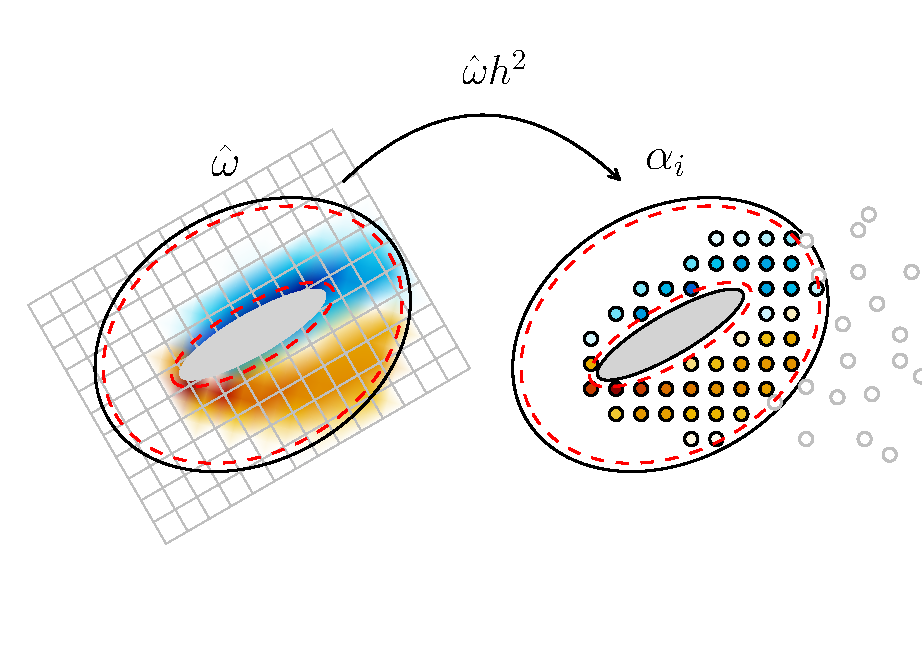
\includegraphics[trim=0.1cm 2.1cm 0.1cm 0.8cm,clip, width=\linewidth]{./figures/coupling/assignStrength/interpolation_StructuredGrid2Blobs-crop.pdf}
		\caption{Bilinear interpolating the strengths from the structured grid SG onto the vortex blobs using equation \ref{eq:coupling-interpolationtoblobs}}
		\label{fig:interpolation_StructuredGrid2Blobs}
		\end{figure}	
	
	\item \textbf{Interpolate the vorticity from $SG$ onto the particle}: Finally, we can solve equation 		\ref{eq:coupling-interpolationtoblobs} to interpolate the vorticity from the nodes of the structured grid onto the pre-generated particle positions. Once we know the vorticity at their position, we can use equation \ref{eq:coupling-standardInitialization} to assign the strengths of the particles. These particles will then have a total circulation of $\hat{\Gamma}_{I}^{L,k}$ according to equation			\ref{eq:coupling-sumparticlestrengths}. Figure \ref{fig:interpolation_StructuredGrid2Blobs} depicts the transfer of the Eulerian solution from the structured grid onto the particle.
	%	
	%	The strengths of the particles are determined
	%	
	%	Figure ?? \ref{fig:interpolation_StructuredGrid2Blobs} depicts the transfer of the vorticityThe vorticity from $SG$ is interpolated onto the positions of the particle using a bilinear interpolation algorithm. The bilinear interpolation of the vorticity is given as,
	%
	%
	%	where $q$ are the vertices of the cells, equation \ref{eq:coupling-eq222}, and is where the vorticity is known. Therefore to perform the interpolation we need to determines the weights $W_q$,
	%
	%
	%	where $\hat{x}$ and $\hat{y}$ are the normalized positions inside its cell, such that $0\leqslant\hat{x}\leqslant\Delta x$ and $0\leqslant\hat{y}\leqslant\Delta y$.
		
	\end{enumerate}
	
	However, as we described in section \ref{seec:coupling-mthlcs}, we must still determine the vortex sheet strengths that satisfied a no-slip boundary condition and ensure conservation of circulation in the domain $\Omega_{in}^k$ due to the correction.

		
	%%	Figure ?? shows the depiction of the algorithm for assigning the strengths of the particles. We see that unlike steps 2 and steps 3, we do not require a point-in-polygon test to determine in which cells of the structured grid $SG$, the newly generated particles reside. As the structured grid $SG$ with equally sized cells with dimension $\Delta x= \Delta y$, we could perform simple algebraic calculations to determine the position of the blobs. Therefore this step, in conjunction with steps 1 to 3, drastically improves the computational efficiency of interpolating the strengths from the Eulerian grid $EG$ onto the newly generated particles $\hat{\mathcal{P}}_{in}$.
		
			
	
	\subsection{Correct Total Circulation}
	
	In this step, we will determine the strengths of the vortex sheet and the total circulation of newly generated vortex particles inside the correction region $\Omega_{in}^k$ such that the circulation conserved during the Lagrangian correction step. The algorithm is however depended on whether the problem is unbounded (without wall boundaries), or bounded (with wall boundary). If we do not have a wall boundary, the step to determine the vortex sheet is not applicable because there exists no vortex sheet.
	
	The algorithm for correcting the total circulation inside $\Omega_{in}^k$ is as follows:
	\begin{enumerate}[label=5.\alph*)]
	\item \textbf{Determine the strengths of the panels} (with solid wall): The total strength of the vortex panels $\Gamma_{\gamma}^{L,k}$ is determined from equation	\ref{eq:coupling-panelstrength}. The Eulerian circulation $\Gamma_{in}^{E,k}$ is the circulation within the boundary $\Sigma_{o}^k$ (see Figure \ref{fig:domainDecomposition_correctionDomains}) and also includes the circulation within the Eulerian body $\Omega_b$. In the case of a moving boundary, there exists a non-zero circulation within the body. The circulation $\Gamma_{I}^{L,k}$ is determined from step 4.d and represents the total circulation of the newly generated vortex particles inside the domain $\Omega_I^k$. Once we determine the required strength for the vortex sheet $\Gamma_{\gamma}^{L,k}$ for all the $k$ Eulerian domains, we can use the approach described in section \ref{sec:boundaryConditions} to solve the multi-body vortex panel problem, satisfy the no-slip boundary condition.

	\item \textbf{Correct the strengths of particles to conserve circulation}: The final step of the \textit{modified Lagrangian correction} algorithm is to ensure conservation of total circulation. This can be achieved by determining the adjusting the strengths of particles $\tilde{\alpha}_p$ using equation \ref{eq:coupling-particlestrengths}. Note that, in case we have unbounded problem, we have the strength of the vortex sheet $\Gamma_{\gamma}^{L,k} = 0$.
	\end{enumerate} 
	

\newpage
\section{Determining Eulerian Substep Boundary Conditions}	
\label{sec:coupling-desbc}

In this section, we elaborate the methodology for determining the Eulerian boundary conditions from the evolved solution of the Lagrangian method. Furthermore, we will explain how to determine the boundary conditions for the substeps of the evolution.

	\begin{figure}[H]
		\centering
		\begin{tikzpicture}
			[node distance=.8cm, start chain=going below,]
			\node[punktchainO, join] (correct) {\textsf{Correct Lagrangian}};
		    \node[punktchainO, join] (evolveL) {\textsf{Evolve Lagrangian}};
		    \node[punktchainS, join] (bcE)     {\textsf{\textbf{Determine Eulerian \\boundary conditions}}};
		    \node[punktchainO, join] (evolveE) {\textsf{Evolve Eulerian}};
		\end{tikzpicture}
		\caption{Flowchart of the hybrid evolution, focusing on the $3^{\mathrm{rd}}$ step: Determine the Eulerian boundary conditions.}
		\label{fig:flowchart_simpleCoupling_}
	\end{figure}

We can determine the Dirichlet velocity boundary condition at the Eulerian boundary $\partial \Omega_E$ from the Lagrangian vorticity field $\omega$ at $t_{n+1}$. The velocity at the Eulerian boundary $\mathbf{x}_{bdry}$ is given by,
\begin{equation}
\mathbf{u}(\mathbf{x}_{i},t_{n+1}) = \sum_p \mathbf{K}_{\sigma}[\mathbf{x}_{i} - \mathbf{x}_p(t_{n+1})]\alpha_p(t_{n+1}),
\end{equation}
where $\mathbf{x}_{}$ are the coordinates of the nodes of the Eulerian mesh that lie in the boundary $\Sigma_d$, as shown in figure \ref{fig:eulerianDirichletBC2}.

	\begin{figure}[!h]
	\centering
	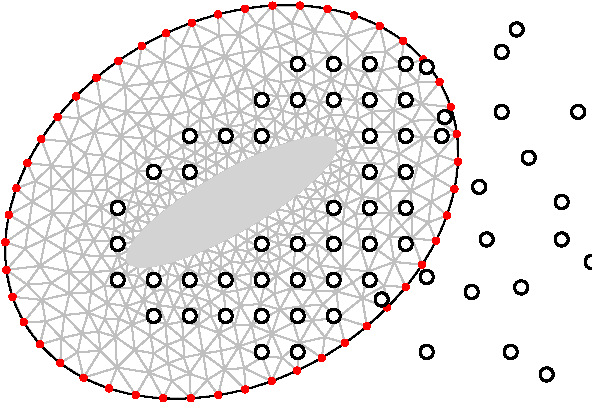
\includegraphics[width=0.5\linewidth]{./figures/hybrid/dirichlet/eulerianDirichletBC-crop.pdf}
	\caption{Dirichlet boundary conditions at boundary of Eulerian domain $\Sigma_d$. We evaluate the induced velocities from the Lagrangian solution at the nodes $\mathbf{x}_i\in\Sigma_d$ [{\color{plotRed}{$\bullet$}}, red dot].}
	\label{fig:eulerianDirichletBC2}
	\end{figure}	


\subsection{Multi-step evolution}
\label{subsec:mse2}
% Evolution, neglect the pressure b.c, and evolve the problem
% sub
In section \ref{subsec:hybrid-ca}, we defined the Eulerian time step $\Delta t_E$ and the Lagrangian time step, such that $\Delta t_E \leqslant \Delta t_L$. The main advantage of this different time step size is that the wake region, where the Lagrangian solver lies, can now be evolved with a much larger time step size.

We perform $k_E$ Eulerian substeps within one Lagrangian time step $t_{n+1}$,
\begin{equation}
t_n^k = t_n + k\Delta t_E,
\end{equation}
where $k = \{0,...,k_E\} \subset \mathbb{N}_0$, and is given by,
\begin{equation}
k_E = \frac{t_{n+1}-t_{n}}{\Delta t_E} = \frac{\Delta t_L}{\Delta t_E}.
\label{eq:timeStepDependency2}
\end{equation}

and we require that $\Delta t_L$ is a multiple of $\Delta t_E$. When $k=0$, we have $t_n^0 = t_n$ and when $k=k_E$, we have $t_n^{k_E} = t_{n+1}$. Figure \ref{fig:multiStep2} depicts the multi-stepping of the Eulerian solution from $t_n^0$ to $t_{n}^{k_E}$ to match the Lagrangian time. As the Eulerian solver requires boundary conditions at each substep, we have to perform an interpolation of the boundary conditions for each substep $t_{n}^k$. We can perform a linear interpolation of the boundary condition in order to determine the boundary conditions at each sub-step,
\begin{equation}
\mathbf{u}(t_n^k) = \mathbf{u}(t_n) + k \Delta \mathbf{u},
\end{equation}
where $\Delta \mathbf{u}$ is given as
\begin{equation}
\Delta \mathbf{u} = \frac{\mathbf{u}(t_{n}^{k_E})-\mathbf{u}(t_n^k)}{k_E},
\end{equation}
and is a linear variation of the velocity between each substep.

	\begin{figure}[!b]
	\centering
	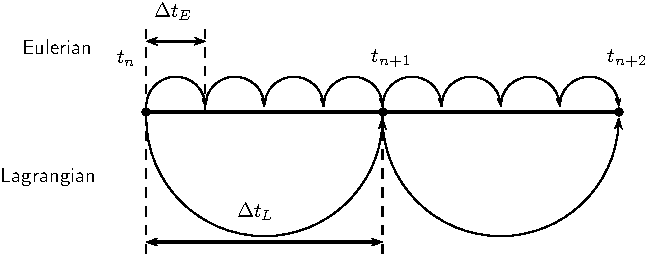
\includegraphics[width=0.7\linewidth]{./figures/eulerian/multiStep-crop.pdf}
	\caption{Eulerian multi-stepping to match the Lagrangian time step. The figure shows $\Delta t_L = 4 \Delta t_E$ and requires $k_E = 4$ Eulerian substeps to time march from $t_n$ to $t_{n+1}$.}
	\label{fig:multiStep2}
	\end{figure}

Once that we have the boundary condition for each of the Eulerian substeps, we can use the approach described in section \ref{sec:eu-eotem} to evolve the Eulerian method from $t_{n}$ to $t_{n+1}$ using $k_E$ Eulerian substeps.


% The evolution of the Eulerian solution is summarized as follows:
%\begin{itemize}
%\item The Eulerian solver uses a $1^{st}$ order Forward Euler time-marching scheme to evolution the solution from $t_n$ to $t_k$.
%\item The solution is evolved $k_E$ steps to reach $t_{n+1}$.
%\item We use velocity-pressure $\mathbf{u}-p$ formulation for the solution in the Eulerian solver.
%\item At the end of the time-step $t_{n+1}$, the Eulerian solver will have a higher resolved solution of the wall-region in comparison to the Lagrangian solver.
%\end{itemize}








	
	
	


